\section{Метод сопряженных градиентов}

\textbf{Алгоритм метода}:
$$ x^{k+1} = x^{k} + t_{k}d^{k}$$

$$ d^{0} = - \nabla f(x^{0})$$
$$ d^{k} = - \nabla f(x^{k}) + \beta_{k - 1}d^{k - 1}$$
$t_{k}$ --- шаг вычисляется из условия наибольшего убывания функции в точках последовательности: $t_{k} = argmin|f(x^{k+1})|$


Основной критерий окончания метода:$|| \nabla f(x^{k})|| < \varepsilon$.

Начальные параметры метода: $x^{0}, \varepsilon$.

Изменяемые параметры метода: отрезок для уточнения шага $[a, b]$.

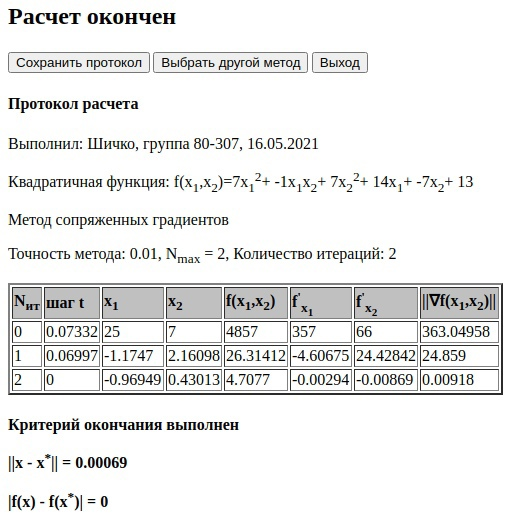
\includegraphics[width=0.8\linewidth]{images/1_prot.jpg}\\
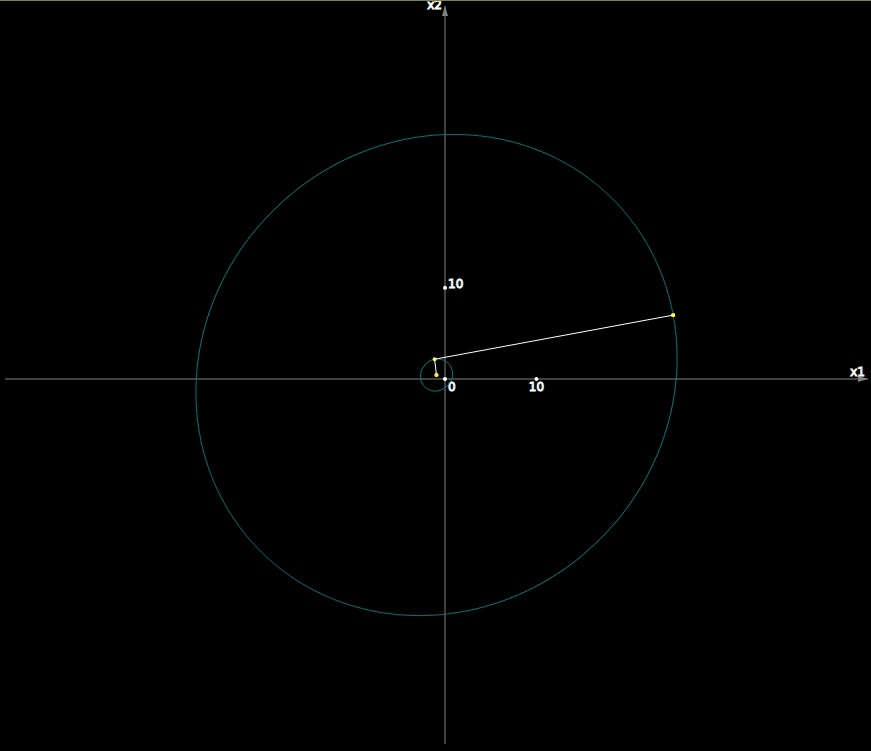
\includegraphics[width=0.6\linewidth]{images/1_image.jpg}\\

\textbf{Последняя итерация}:

$x^{0}_{1} = N^{0} = 25$\\
$x^{0}_{2} = 7$\\
$x^{2} = x^{1} + t_{1} +d^{1}$\\
$
x^{1} = 
\begin{pmatrix}
  -1.1747\\
  2.16098
\end{pmatrix}
$\\
$t_{1} = 0.06997$\\
$d^{1} = -\nabla f(x^{1}) + B_{0}d^{0}$\\
$d^{0} = -\nabla f(x^{0})$\\
$B_{0} = \dfrac{||\nabla f(x^{1})||^{2}}{||\nabla f(x^{0})||^{2}} = \dfrac{(24.859)^{2}}{(363.04958)^{2}} = 0.0033$\\
$
\nabla f = 
\begin{pmatrix}
  14x_{1} - x_{2} + 14\\
  14x_{2} - x_{1} - 7
\end{pmatrix}
$\\
$
\nabla f(x^{0}) = 
\begin{pmatrix}
  357\\
  66
\end{pmatrix}
$\\
$
\nabla f(x^{1}) = 
\begin{pmatrix}
  -4.60675\\
  24.42842
\end{pmatrix}
$\\
Тогда\\
$
d^{1} = 
\begin{pmatrix}
  4.60675\\
  -24.42842
\end{pmatrix}
+
\begin{pmatrix}
  -0.3003\\
  -0.2805
\end{pmatrix}
=
\begin{pmatrix}
  4.30645\\
  -24.70892
\end{pmatrix}
$\\

$
x^{2} = 
\begin{pmatrix}
  -1.1747\\
  2.16098
\end{pmatrix}
+ 0.06997
\begin{pmatrix}
  4.30645\\
  -24.70892
\end{pmatrix}
=
\begin{pmatrix}
  -0.966949\\
   0.43013
\end{pmatrix}
$

\pagebreak
